\documentclass{article}
\usepackage{fancyhdr}
\usepackage{setspace}
\usepackage{titlesec}
\usepackage[style=apa, sorting=nyt]{biblatex}
\usepackage{geometry}
\usepackage{hyperref}
\usepackage{xurl}
\usepackage{enumitem}
\usepackage{tabularx}
\usepackage{xltabular}
\usepackage{graphicx}
\usepackage{float}
\usepackage{caption}

\geometry{a4paper, margin=1in}
\renewcommand{\arraystretch}{1.5}
\captionsetup[figure]{skip=4pt}
% \addbibresource{references.bib}

\begin{document}

% ---------- Cover page ----------
\begin{titlepage}
\begin{center}
\vspace*{1cm}

Swinburne University of Technology \\
School of Science, Computing, and Emerging Technologies
\vspace{8cm}

COS40005 - Computing Technology Project A \\
Project: UG\_COSEAT\_02 - Developing an AI Tool for Automated Building Management System Functional Compliance Verification Using Large Language Models and Knowledge Graphs \\
\vspace{1em}
\textbf{Contribution Summary} \\
\textbf{Contribution for the Planning Phase}
\vfill

Student name: Ngoc Van Nhi Do \\
Student ID: 105551765 \\
Submission date: 16/09/2026
\end{center}
\end{titlepage}

% ---------- Header + footer ----------
\pagestyle{fancy}
\fancyhead[L]{Ngoc Van Nhi Do}
\fancyhead[R]{105551765}
\fancyfoot{}
\renewcommand{\footrulewidth}{0.4pt} % default is 0pt
\fancyfoot[L]{COS40005 - Computing Technology Project A}
\fancyfoot[R]{\small\thepage}

% \tableofcontents
% \newpage

\begin{center}
\vspace*{2px}
{\Large
\setlength{\baselineskip}{2em}
Planning Phase Contribution Summary
}
\end{center}

\section*{Acknowledgement of Country}

I respectfully acknowledge the Wurundjeri People of the Kulin Nation, who are the Traditional Owners of the land on which Swinburne's Australian campuses are located in Melbourne's east and outer-east, and pay my respect to their Elders past, present and the emerging.

\section{Contribution Evidence and Impact}

\subsection{Overview}

Table~\ref{tab:contribution-summary} summarises the main tasks that I have completed throughout the initial planning phase of the project.

\begin{xltabular}{\textwidth}{X p{2cm} p{1.5cm} p{5cm}}
\caption{Contribution Summary}
\label{tab:contribution-summary} \\
\hline
\textbf{Task} & \textbf{Assignment} & \textbf{Time spent} & \textbf{Evidence} \\
\hline
\endfirsthead

\hline
\endlastfoot

Team organisation and coordination & Self-assigned & 0.25 hours & Canvas discussions, Discord discussions \\

Project onboarding and stakeholder communication & Self-assigned & 1 hour & Discord discussions, emails \\

Trello board setup and organisation & Self-assigned & 0.5 hours & Trello board \\

Project journal and meeting documentation & Assigned & 4 hours & Documentation \\

Solution research & Self-assigned & 30 hours & Research notes, Discord discussions, individual research report \\

PDF parsing and extraction experiments & Self-assigned & 6 hours & Personal GitHub repository \\

Week 6 demonstration preparation & Assigned & 5 hours & Discord discussion, presentation slides \\

Solution design & Assigned & 10 hours & Discord discussions, research notes, documentation \\

Team and Project Plan development and submission & Assigned & 8 hours & Discord discussions, documentation \\

\hline

\textbf{Total time spent on the project} & & \textbf{64.75 hours} & \\

\end{xltabular}

\subsection{Contributions in Detail}

\subsubsection*{Contribution 1 - Team Organisation and Coordination}

    \begin{xltabular}{\textwidth}{p{2cm} X}
    \caption{Contribution 1 Details} \\
    \hline
    \textbf{STAR} & \textbf{Description} \\
    \hline
    \endfirsthead

    \hline
    \endlastfoot

    \textbf{Situation} & After enrolling in the project, I only realised by Thursday that I hadn't yet connected with my team or set up a communication channel, which needed to be done as soon as possible if the team wanted to conduct a supervisor meeting by the end of the week. \\

    \textbf{Task} & Get in touch with my teammates and establish a shared communication channel. \\

    \textbf{Action} & I posted a new discussion on our team project page, introduced myself, and asked for everybody's contact details so we could set up a shared channel. The team agreed on Discord, so I created a server and added the whole team. \\

    \textbf{Result} & I got to know my teammates, their backgrounds and areas of expertise, and we had an official team channel up and running to get the project started. \\

    \end{xltabular}

    \begin{figure}[H]
    \centering
    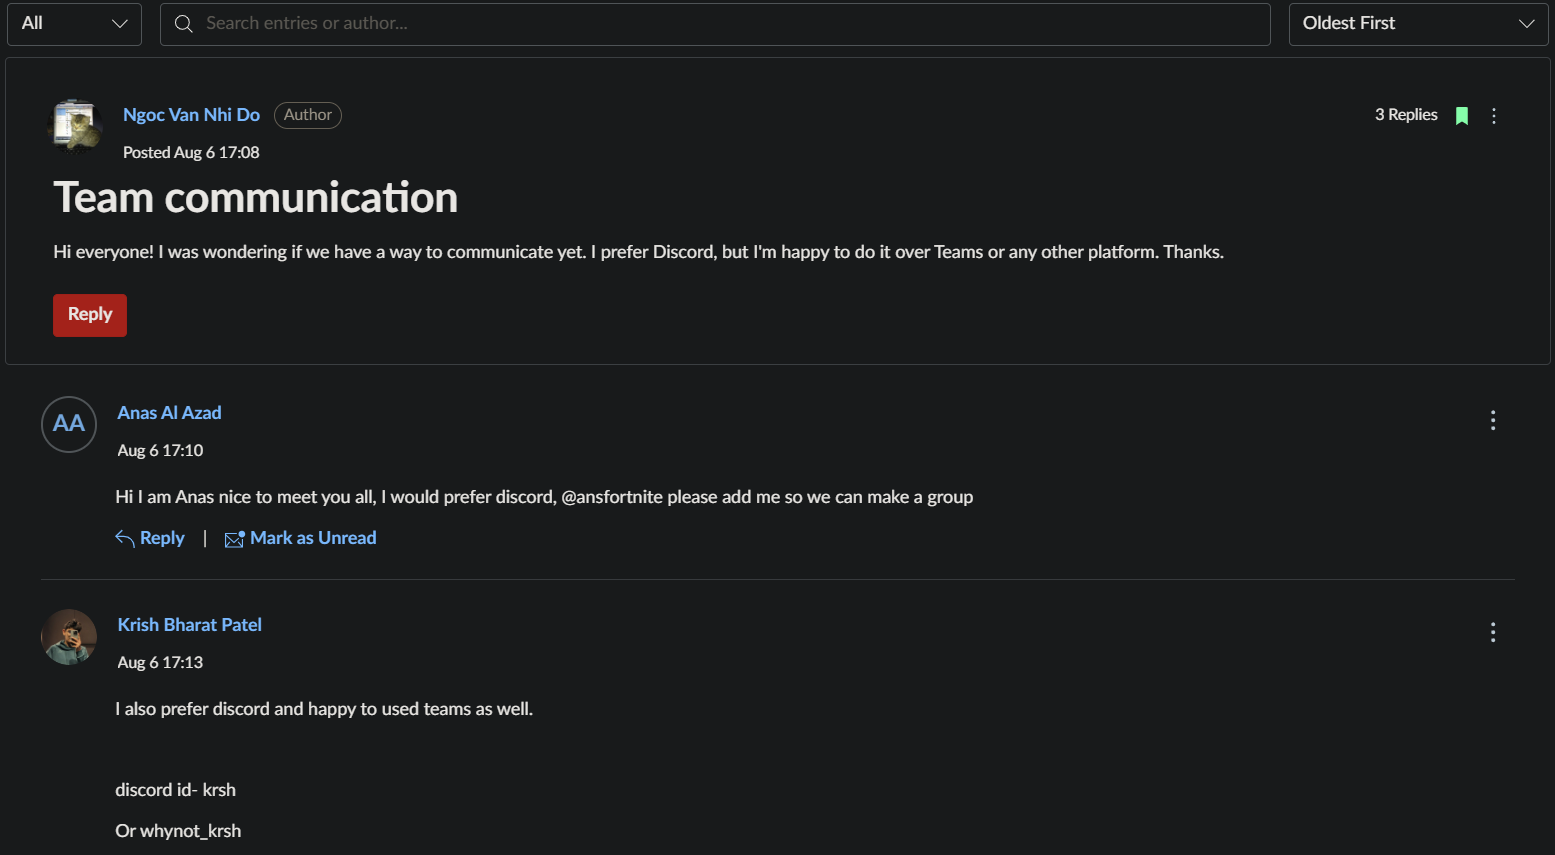
\includegraphics[scale=0.4]{images/1_canvas.jpg}
    \caption{My message on the Team page on Canvas.}
    \end{figure}

    \begin{figure}[H]
    \centering
    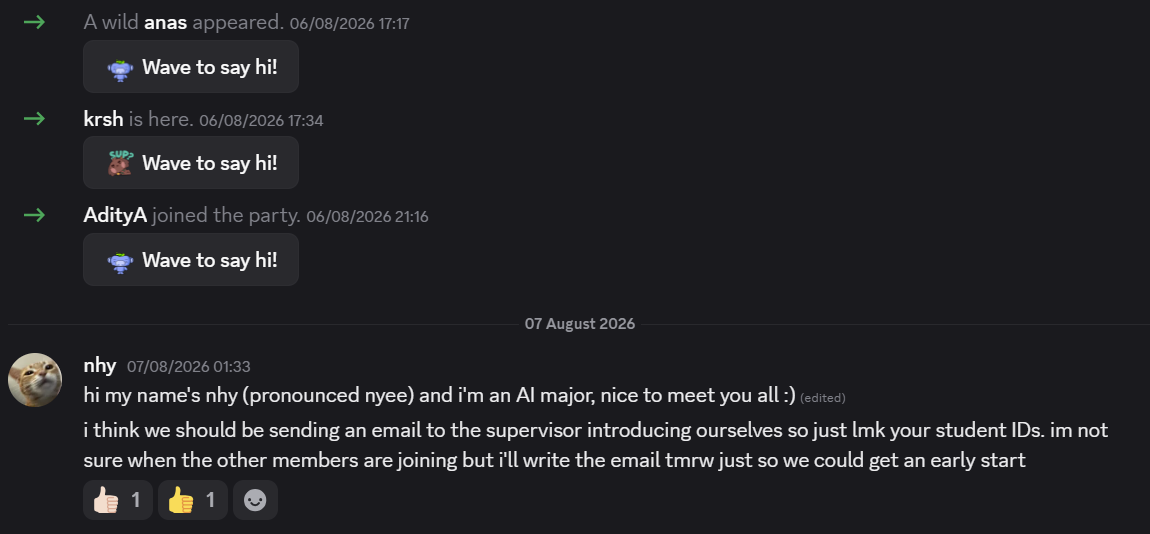
\includegraphics[scale=0.5]{images/1_introduction.jpg}
    \caption{I added everybody to a Discord server and introduced myself.}
    \end{figure}

\subsubsection*{Contribution 2 - Project Onboarding and Stakeholder Communication}

    \begin{xltabular}{\textwidth}{p{2cm} X}
    \caption{Contribution 2 Details} \\
    \hline
    \textbf{STAR} & \textbf{Description} \\
    \hline
    \endfirsthead

    \hline
    \endlastfoot

    \textbf{Situation} & We needed to contact our supervisor as soon as possible to arrange a meeting by the end of the week. We also needed to get the client's details to learn more about the project and get started. \\

    \textbf{Task} & Introduce our team to the supervisor, and then, once we had the client's details, introduce the team to the client. \\

    \textbf{Action} & I emailed the supervisor to request a meeting by the end of the week and ask for the client's details. Meanwhile, I pulled the client introduction template from Canvas, wrote the introduction, and had each team member fill in their details. Once the client's details came through, I sent the introduction email and arranged a meeting time with him. \\

    \textbf{Result} & The team and the supervisor agreed to meet on Friday of Week 1, 6:30-7:30 pm. After getting the client's details, I arranged our first meeting with him for the following Tuesday at 5:00 pm. \\

    \end{xltabular}

    \begin{figure}[H]
    \centering
    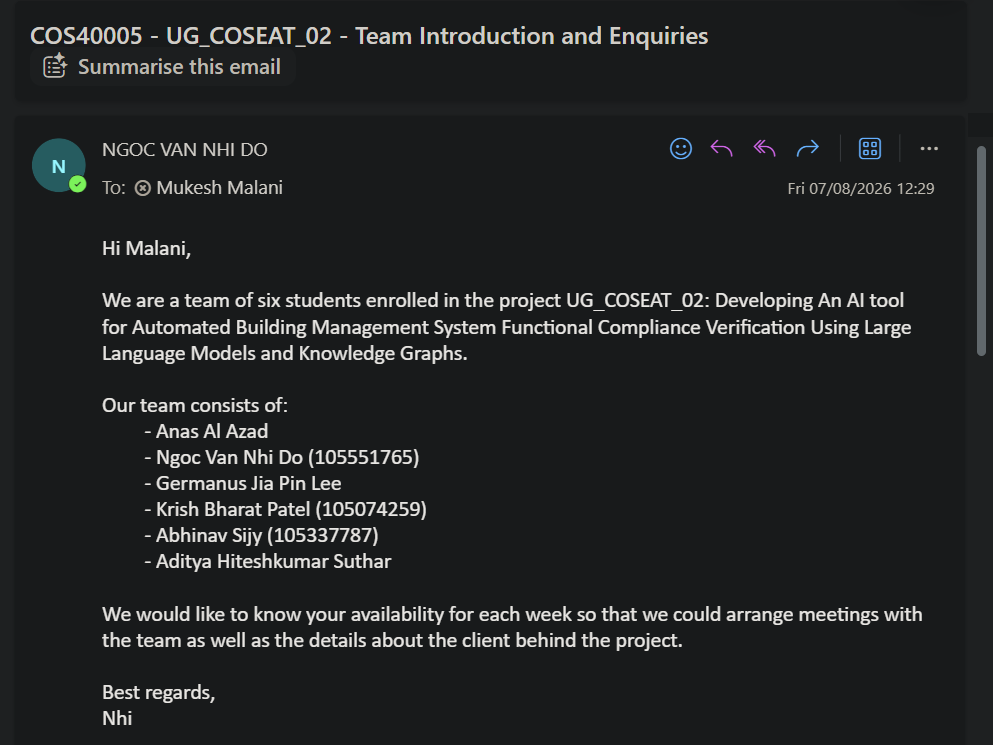
\includegraphics[scale=0.5]{images/2_supervisor_email.jpg}
    \caption{I emailed our supervisor to introduce the team, requesting availability for the weekly supervisor meeting and client details.}
    \end{figure}

    \begin{figure}[H]
    \centering
    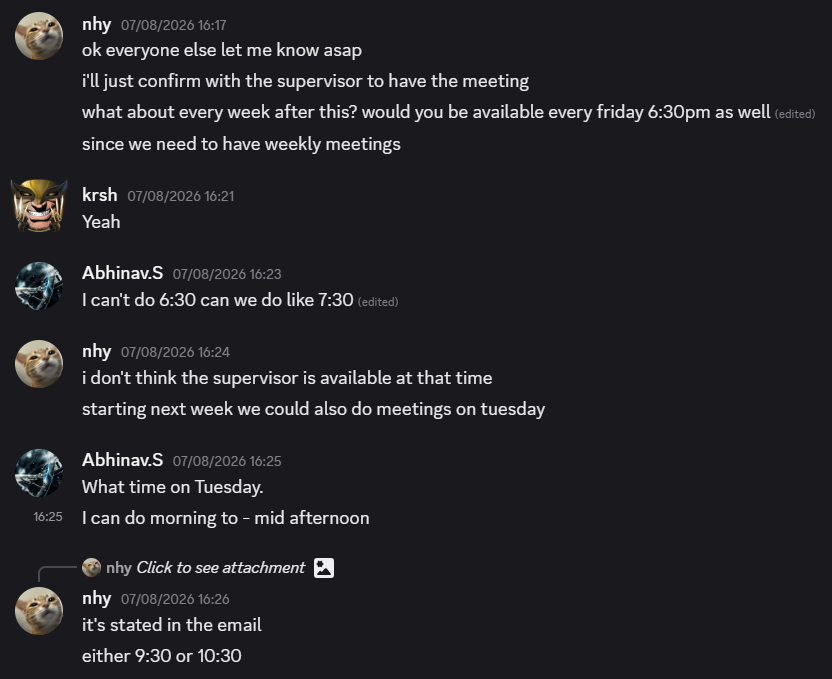
\includegraphics[scale=0.6]{images/2_arrange_meeting.jpg}
    \caption{I helped the team arrange a meeting time for Week 1 and subsequent weekly meeting times.}
    \end{figure}

    \begin{figure}[H]
    \centering
    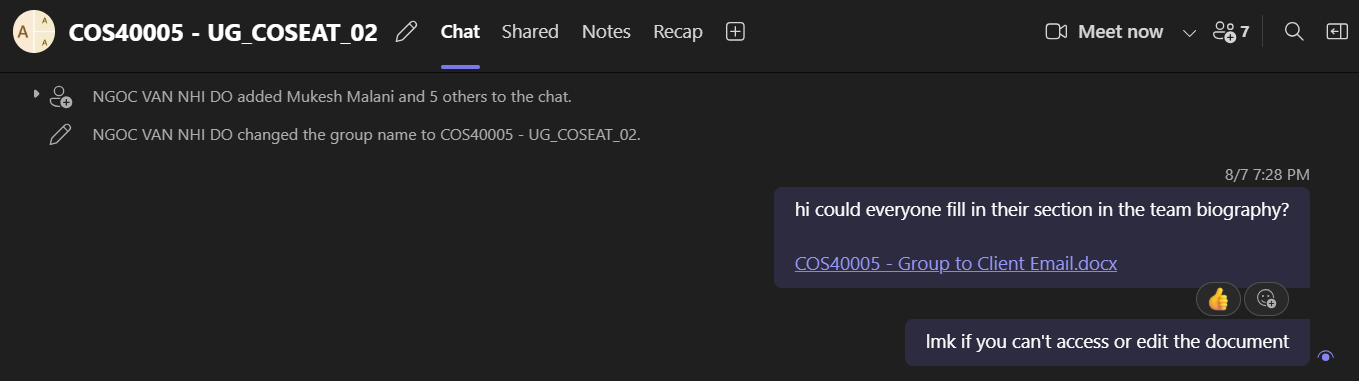
\includegraphics[scale=0.5]{images/2_client_template.jpg}
    \caption{I asked the team to fill in their biographies for the client email.}
    \end{figure}

    \begin{figure}[H]
    \centering
    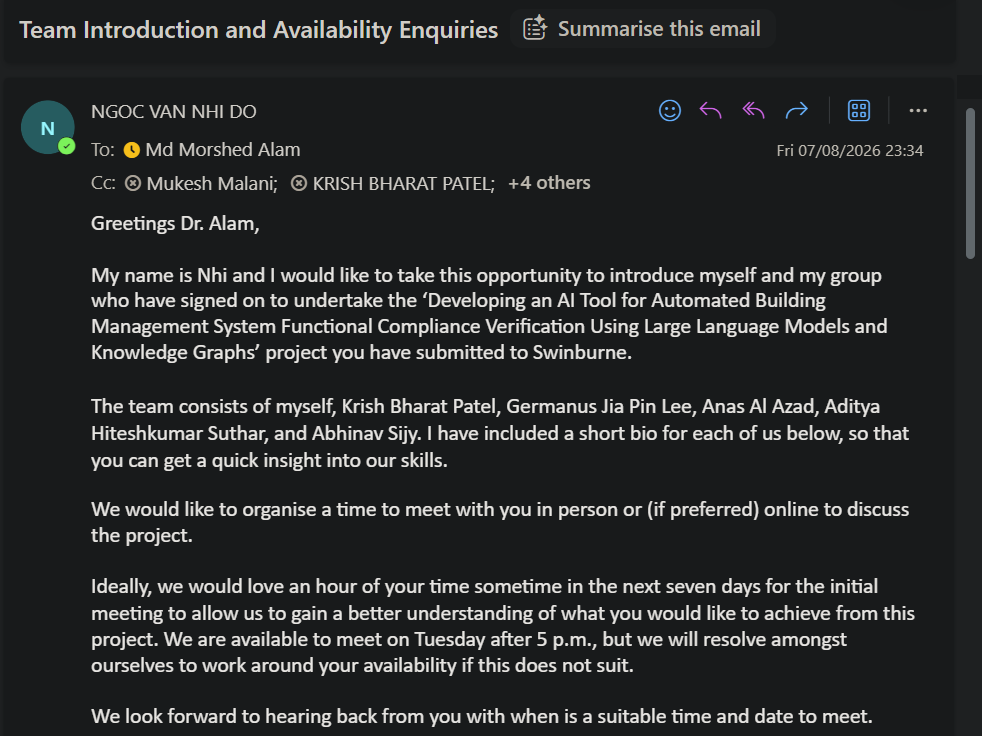
\includegraphics[scale=0.5]{images/2_client_email.jpg}
    \caption{I sent the email on behalf of the team to introduce ourselves and arrange a meeting time.}
    \end{figure}

\subsubsection*{Contribution 3 - Trello Board Setup and Organisation}

    \begin{xltabular}{\textwidth}{p{2cm} X}
    \caption{Contribution 3 Details} \\
    \hline
    \textbf{STAR} & \textbf{Description} \\
    \hline
    \endfirsthead

    \hline
    \endlastfoot

    \textbf{Situation} & The team needed to set up a project management tool for our project as a way to keep track of tasks and also to store important notes and documentation. \\

    \textbf{Task} & Have a project management tool set up and shared with everybody, and create a structure on the shared workspace so that it's organised and easy to navigate. \\

    \textbf{Action} & I asked the team for their preferences on a project management tool and suggested Trello, based on a friend's recommendation, for its simplicity and clean interface. Once Krish created the board, I set up the initial list structure and added cards to store what we had discussed so far. \\

    \textbf{Result} & The team now has a structured project management workspace, making it easy to track tasks, store notes, manage deadlines, and stay aligned on project progress. \\

    \end{xltabular}

    \begin{figure}[H]
    \centering
    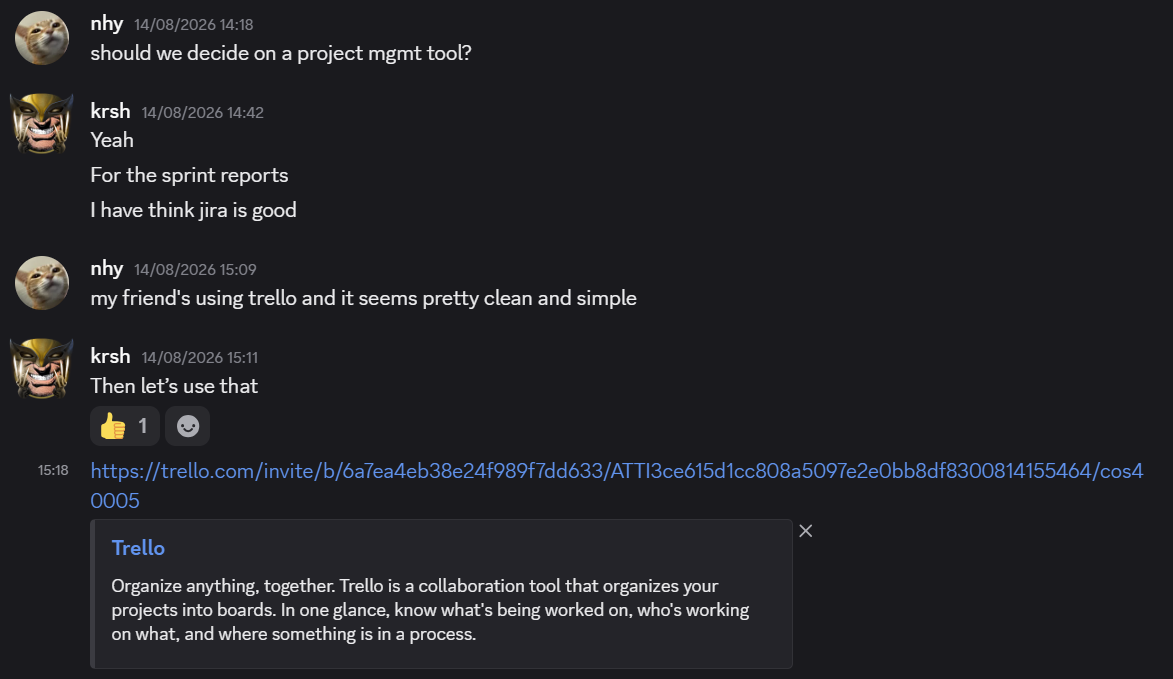
\includegraphics[scale=0.5]{images/3_create_trello.jpg}
    \caption{I reminded the team to set up a project management tool. Krish helped me create the actual board.}
    \end{figure}

    \begin{figure}[H]
    \centering
    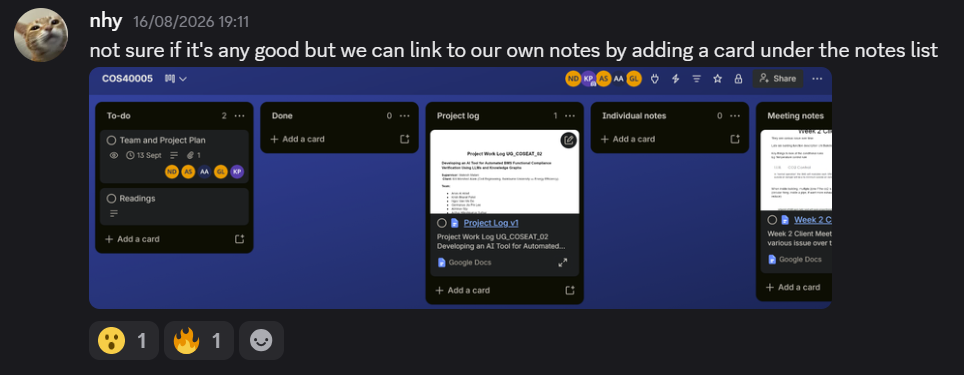
\includegraphics[scale=0.6]{images/3_trello_board.jpg}
    \caption{I created the structure containing lists and cards on the Trello board. This structure would eventually be modified and adapted as the project progresses.}
    \end{figure}

\subsubsection*{Contribution 4 - Project Journal and Meeting Documentation}

    \begin{xltabular}{\textwidth}{p{2cm} X}
    \caption{Contribution 4 Details} \\
    \hline
    \textbf{STAR} & \textbf{Description} \\
    \hline
    \endfirsthead

    \hline
    \endlastfoot

    \textbf{Situation} & Anas suggested we keep a project journal to track our work and progress and record important information for future reference. We also needed to take meeting notes for supervisor, client, and occasional team meetings each week, which we assigned using a roster. \\ 

    \textbf{Task} & Write meeting notes when I'm asked to, and contribute to the project journal. \\

    \textbf{Action} & I wrote meeting notes for Week 3 and Week 6, updated the project journal in Week 3, and occasionally recapped team meetings for members who couldn't attend. \\

    \textbf{Result} & These documents gave the team a reliable reference for what was discussed and decided in each meeting, kept absent members in the loop, and made it easy for us to keep track of the project's progress and direction. \\

    \end{xltabular}

    The project log is not as frequently updated because most of the information we needed to keep track of was already recorded in the meeting notes or posted on the Trello board.

    \begin{xltabular}{\textwidth}{p{4cm} X}
    \caption{Documentation Links} \\
    \hline
    \textbf{Document} & \textbf{URL} \\
    \hline

    Project Log & \url{https://docs.google.com/document/d/161b-WrsadZZaBq0WX-C8wwvEc8AJE8trWAqeaGkFChw/edit} \\
    Week 3 meeting notes & \url{https://docs.google.com/document/d/1WdaFi9pqphsC86g0fr1Vazsp2pVx1C348ypmlM1nFhQ/edit} \\
    Week 6 meeting notes & \url{https://docs.google.com/document/d/15exNUMa88fH8xraCrFS4MbCKsYV2SY9AaO6yHp1tKsk/edit} \\

    \hline
    \end{xltabular}

\subsubsection*{Contribution 5 - Solution Research}

    \begin{xltabular}{\textwidth}{p{2cm} X}
    \caption{Contribution 5 Details} \\
    \hline
    \textbf{STAR} & \textbf{Description} \\
    \hline
    \endfirsthead

    \hline
    \endlastfoot

    \textbf{Situation} & I believe our project is relatively involved as it requires designing a novel pipeline rather than implementing an existing solution for this business scenario. It requires understanding the building and construction domain, as well as researching unfamiliar technologies such as ontologies, RDF, and knowledge graphs. Each member must understand the business requirements, existing solutions, and related research in order to develop a solution, while keeping the whole team on the same page despite running individual research during the first few weeks of the planning phase. \\

    \textbf{Task} & Individually investigate the business and technical domain, review existing solutions and similar research, build an understanding of HVAC concepts and semantic web technologies. \\

    \textbf{Action} & I first focused on understanding the project requirements and constraints, then spent a significant amount of time building domain knowledge to assess the feasibility of my ideas. This included reading research papers (including those sent by the client), studying the methodologies used in existing solutions and how they could be applied to our project, and collecting information through Youtube videos, tutorials, blogs, and journal articles. I documented my findings so I could share them with the rest of the team, and reviewed my teammates' research to identify similarities and differences in our approaches, following up with questions to ensure I understood their ideas well. \\

    \textbf{Result} & I developed a strong grasp of the technology stack which we will be using for the project, along with a clear sense of how the implementation phase will unfold. My proposed ideas were also used as the foundation for our final solution design. \\

    \end{xltabular}

    My individual notes which were shared with the rest of the team can be found at \url{https://docs.google.com/document/d/1efj728WyIx13IP7YUCyFppa7tIOdh86SQdh_qG0e7vU/edit?usp=sharing}. They include notes on basic HVAC concepts, summaries of the three research papers provided by the client, and an initial proposal for the first half of our pipeline, which I developed in Week 3. The full scope of my research is presented in my Individual Research Report and the Solution Approach and Research sections in our Project Plan.

    \begin{figure}[H]
    \centering
    
\includegraphics[scale=0.6]{images/5_research_discussions.jpg}
    \caption{I followed up after reading my teammates' research to gain a better understanding of their proposals.}
    \end{figure}

\subsubsection*{Contribution 6 - PDF Parsing and Extraction Experiments}

    \begin{xltabular}{\textwidth}{p{2cm} X}
    \caption{Contribution 6 Details} \\
    \hline
    \textbf{STAR} & \textbf{Description} \\
    \hline
    \endfirsthead

    \hline
    \endlastfoot

    \textbf{Situation} & As we were implementing a novel solution, I was concerned about the feasibility of the proposed approaches. Since our framework was LLM-based, the team also wanted to run preliminary tests on local and cloud models to gauge their performance on the extraction task. This was originally assigned to Abhinav, but as he didn't have experience setting up a local agent and couldn't complete it in time, I took over so we could get early results and something concrete to show the client. The expectation of showing tangible progress each week, besides formal documentation, also motivated me to develop subsequent experiments in code across Weeks 3, 4, and 5. \\

    \textbf{Task} & Write experimental scripts for the PDF parsing, entity extraction, and logic rule extraction stages to assess the performance of the Docling library and LLM response quality. \\

    \textbf{Action} & I ran three experiments across three weeks. The first assessed how well the \texttt{docling} library could read the Latelab PDF and how the \texttt{llama3.2:1b} model could summarise the extracted information, the second parsed the PDF into a more structured output and extracted entities into a JSON schema, and the third built on the second to extract control logic. I shared the results and the source code with the team each week so they could run their own experiments or build on my code to fix any issues they found. \\

    \textbf{Result} & The experiments revealed model inaccuracies and inconsistencies, which later informed our decision to develop a model-agnostic pipeline. They also confirmed Docling as a reliable PDF parsing tool, and the results were useful in demonstrating our ideas and LLM extraction performance to the client. \\

    \end{xltabular}

    Source code files can be found in my personal GitHub repository for this unit at \url{https://github.com/nhydnv/COS40005-Computing-Technology-Project-A/tree/main/experiments}. Each directory is named after the date when I conducted these experiments.

    \begin{figure}[H]
    \centering
    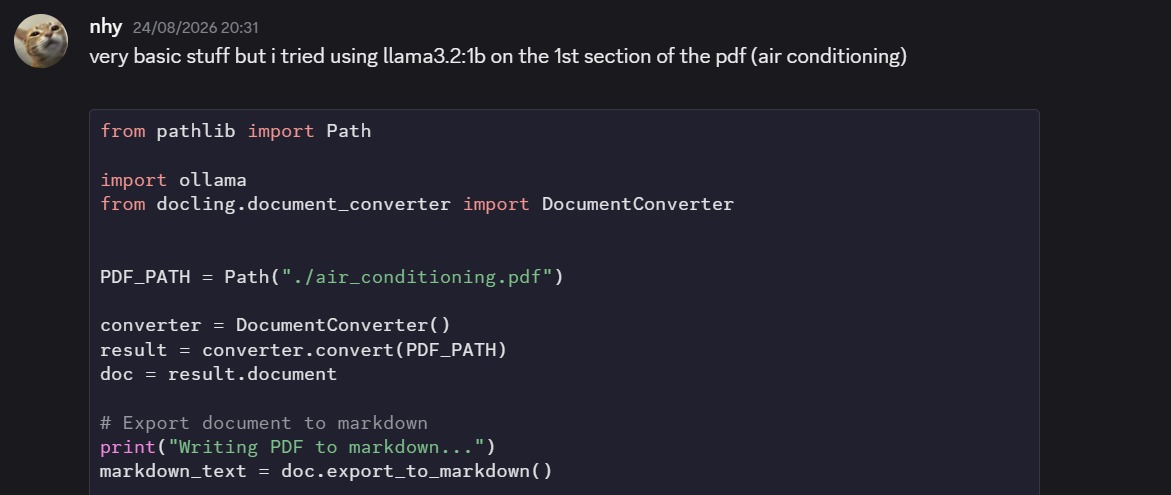
\includegraphics[scale=0.5]{images/6_code_1.jpg}
    \end{figure}
    \begin{figure}[H]
    \centering
    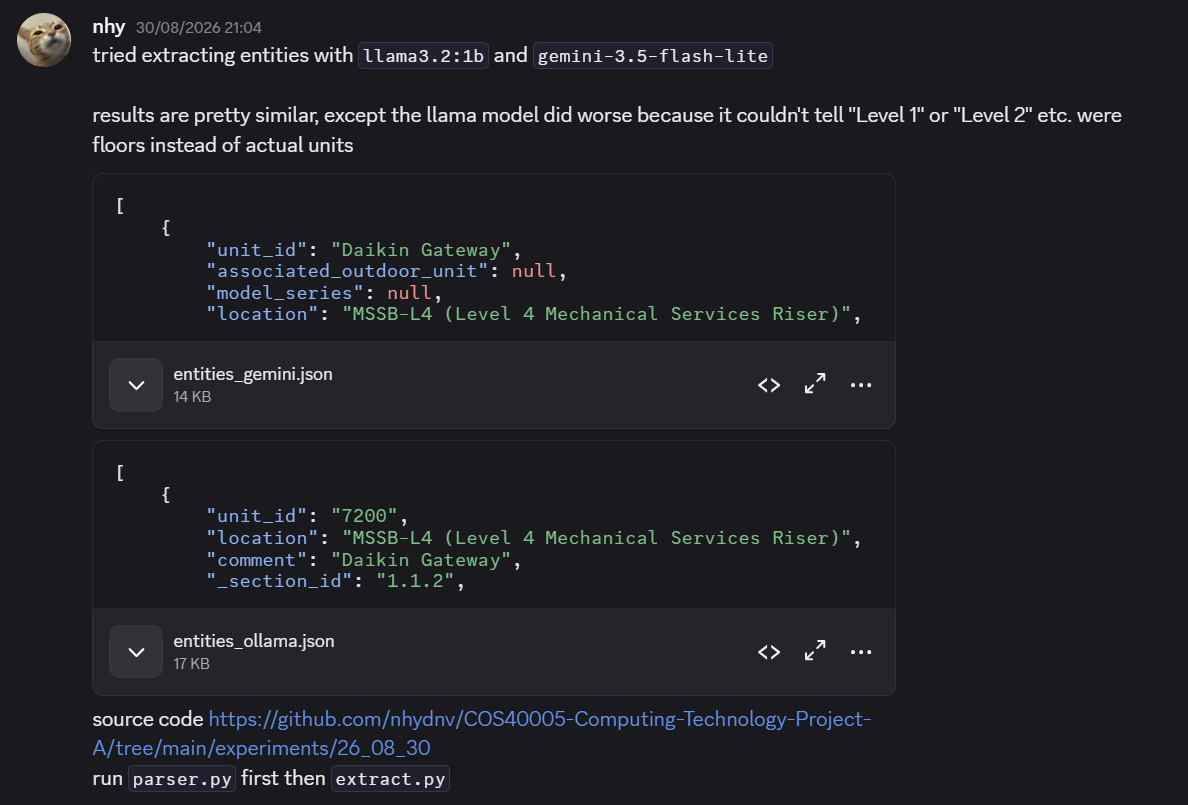
\includegraphics[scale=0.4]{images/6_code_2.jpg}
    \end{figure}
    \begin{figure}[H]
    \centering
    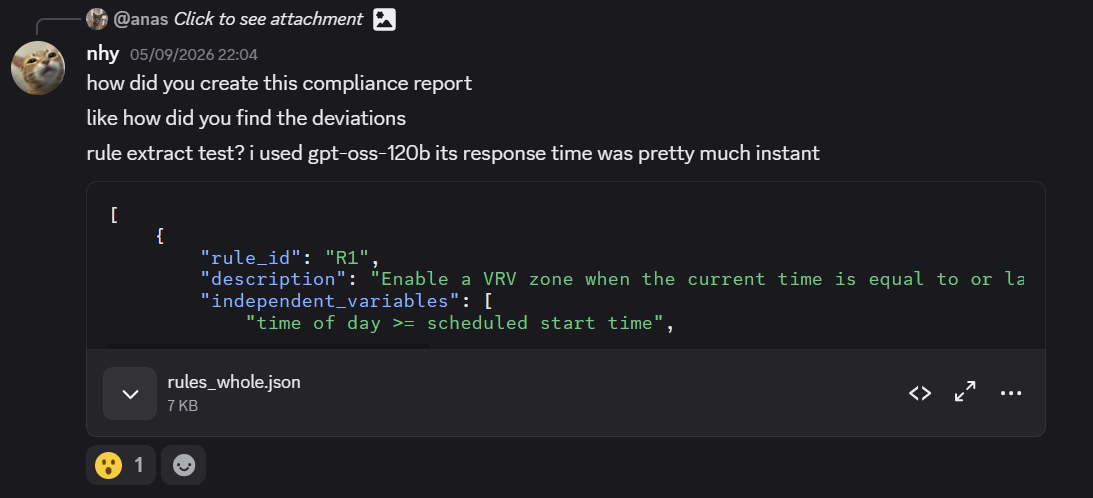
\includegraphics[scale=0.5]{images/6_code_3.jpg}
    \caption{I shared the results of my experiment each week with the rest of the team.}
    \end{figure}

\subsubsection*{Contribution 7 - Week 6 Demonstration Preparation}

    \begin{xltabular}{\textwidth}{p{2cm} X}
    \caption{Contribution 7 Details} \\
    \hline
    \textbf{STAR} & \textbf{Description} \\
    \hline
    \endfirsthead

    \hline
    \endlastfoot

    \textbf{Situation} & We were asked to present our proposed solution approach to the client at our Week 6 Demonstration. I realised the team wasn't entirely on the same page up to this point, with some members still unclear on the scope we'd be covering this semester. We needed a serious discussion about the project plan, architecture, what to prepare for the client demonstration, and the overall team direction. \\

    \textbf{Task} & Host a team meeting, outline the agenda, resolve any uncertainties so the team was aligned, and allocate tasks for each member ahead of the client meeting. \\

    \textbf{Action} & I prepared a list of talking points for the meeting, including the expected scope, this semester's deliverables, the solution architecture, and the proposed technology stack, and hosted the discussion to make sure all bases were covered. I split our tasks into "big tasks" (covering the final solution design) and "small tasks" (covering preparation for the client demonstration the following Tuesday). In a follow-up one-to-one with Anas to finalise our solution approach, I also suggested building a prototype to showcase to the client rather than relying on static slides, which he agreed to and took on. \\

    \textbf{Result} & The team was aligned on the project plan and scope, and we had a clear breakdown of responsibilities heading into the demonstration meeting. \\

    \end{xltabular}

    Week 6 meeting notes (\url{https://docs.google.com/document/d/15exNUMa88fH8xraCrFS4MbCKsYV2SY9AaO6yHp1tKsk/edit}) summarised the meeting which I hosted with the team and the one-to-one discussion I had with Anas.

    \begin{figure}[H]
    \centering
    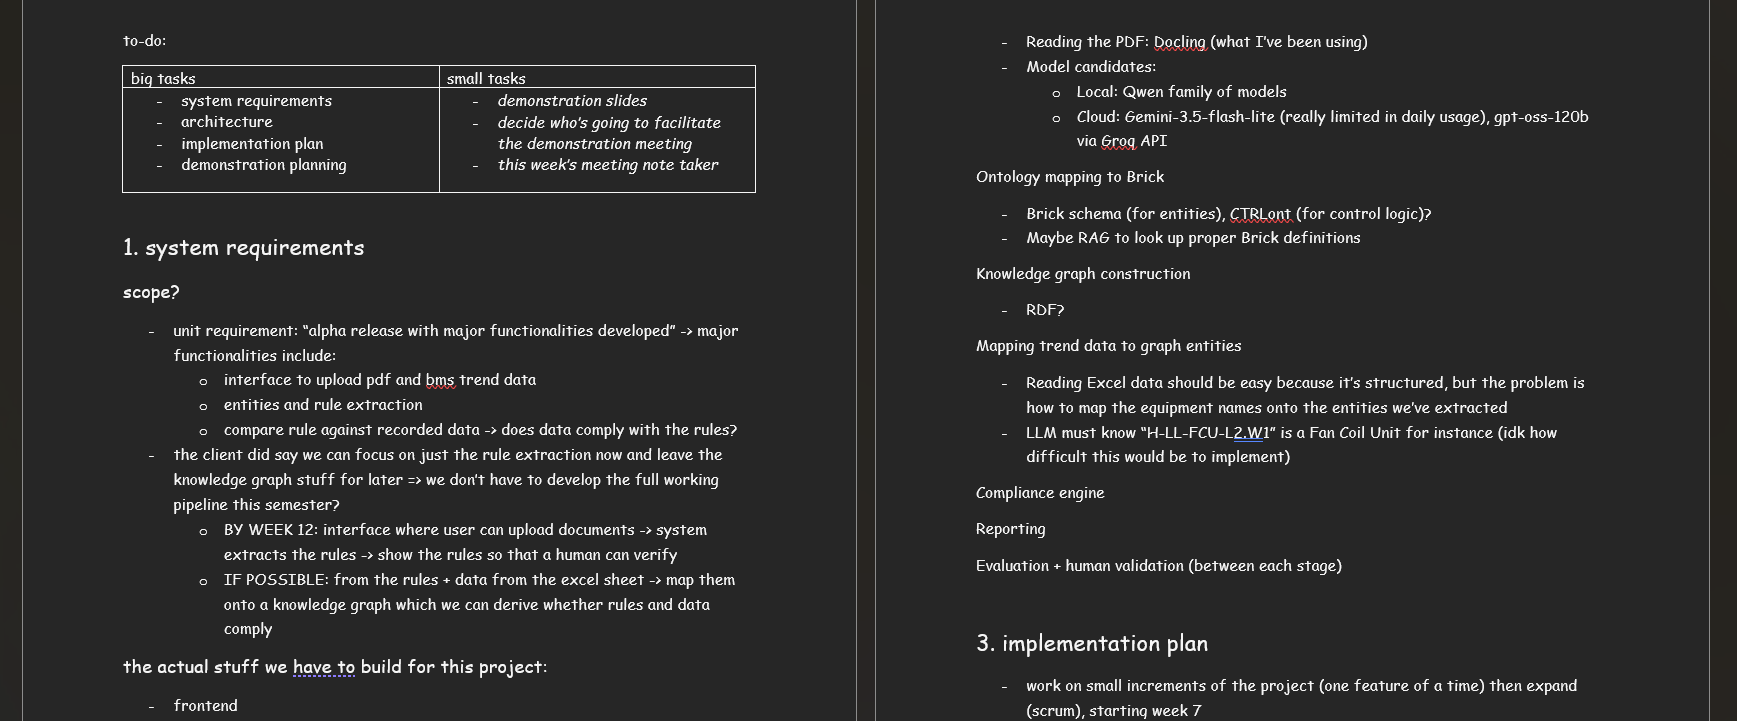
\includegraphics[scale=0.4]{images/7_itinerary.jpg}
    \caption{Snippet of the list of tasks and talking points I had outlined prior to our meeting.}
    \end{figure}

    \begin{figure}[H]
    \centering
    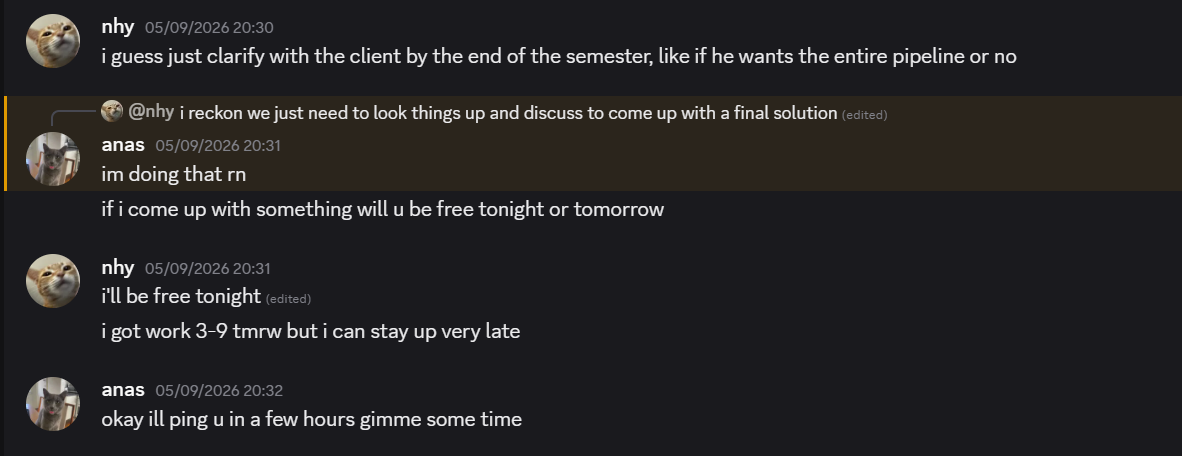
\includegraphics[scale=0.6]{images/7_discussion.jpg}
    \caption{Anas and I agreeing to finalise the solution approach following the first team meeting.}
    \end{figure}

    \begin{figure}[H]
    \centering
    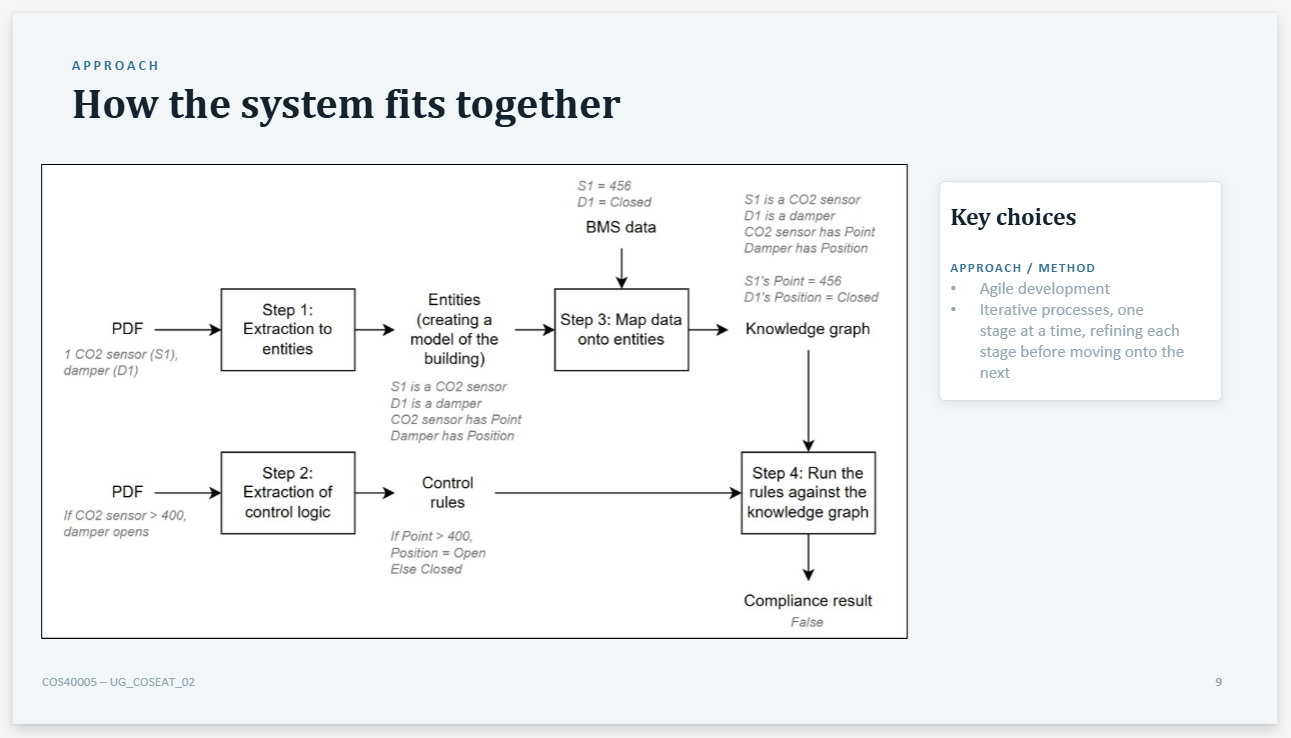
\includegraphics[scale=0.5]{images/7_slide.jpg}
    \caption{The slide I had prepared in our demonstration presentation to illustrate a high-level overview of our proposed architecture.}
    \end{figure}

\subsubsection*{Contribution 8 - Solution Design}

    \begin{xltabular}{\textwidth}{p{2cm} X}
    \caption{Contribution 8 Details} \\
    \hline
    \textbf{STAR} & \textbf{Description} \\
    \hline
    \endfirsthead

    \hline
    \endlastfoot

    \textbf{Situation} & Following the team meeting discussed in Contribution 7, the team still needed to do some additional research to finalise the solution approach. Even though each of us had our own ideas from conducting our individual research, none of the members had a fully realised end-to-end pipeline and thoroughly understood each other's approaches. This called for a thorough review and discussion so that we had a concrete, final high-level system architecture. \\

    \textbf{Task} & Explain my proposed solution to myself and to Anas to check for gaps and ensure we were on the same page. Formalise our research into one unified architecture and workflow, and brainstorm ways to present this architecture to the client. \\

    \textbf{Action} & This responsibility was shared between Anas and me, as the rest of the team didn't have direct input into the final solution approach. Since we were both beginners in semantic web technologies and knowledge graphs, I had Claude generate a beginner-level walkthrough of my proposed pipeline and cross-checked it against original documentation for accuracy, which also served as a learning aid for us. I then tested the pipeline using a simple control logic example (if X then Y) to confirm the workflow makes sense from start to finish. We then combined my approach with Anas's model-agnostic design to arrive at our final solution. \\

    \textbf{Result} & We produced a finalised solution design, along with an interactive demo built by Anas that presented the workflow in a visually engaging and intuitive way. This was showcased at the demonstration meeting and left the client impressed. \\

    \end{xltabular}

    Week 6 meeting notes (\url{https://docs.google.com/document/d/15exNUMa88fH8xraCrFS4MbCKsYV2SY9AaO6yHp1tKsk/edit}) summarised the one-to-one discussion I had with Anas.

    \begin{figure}[H]
    \centering
    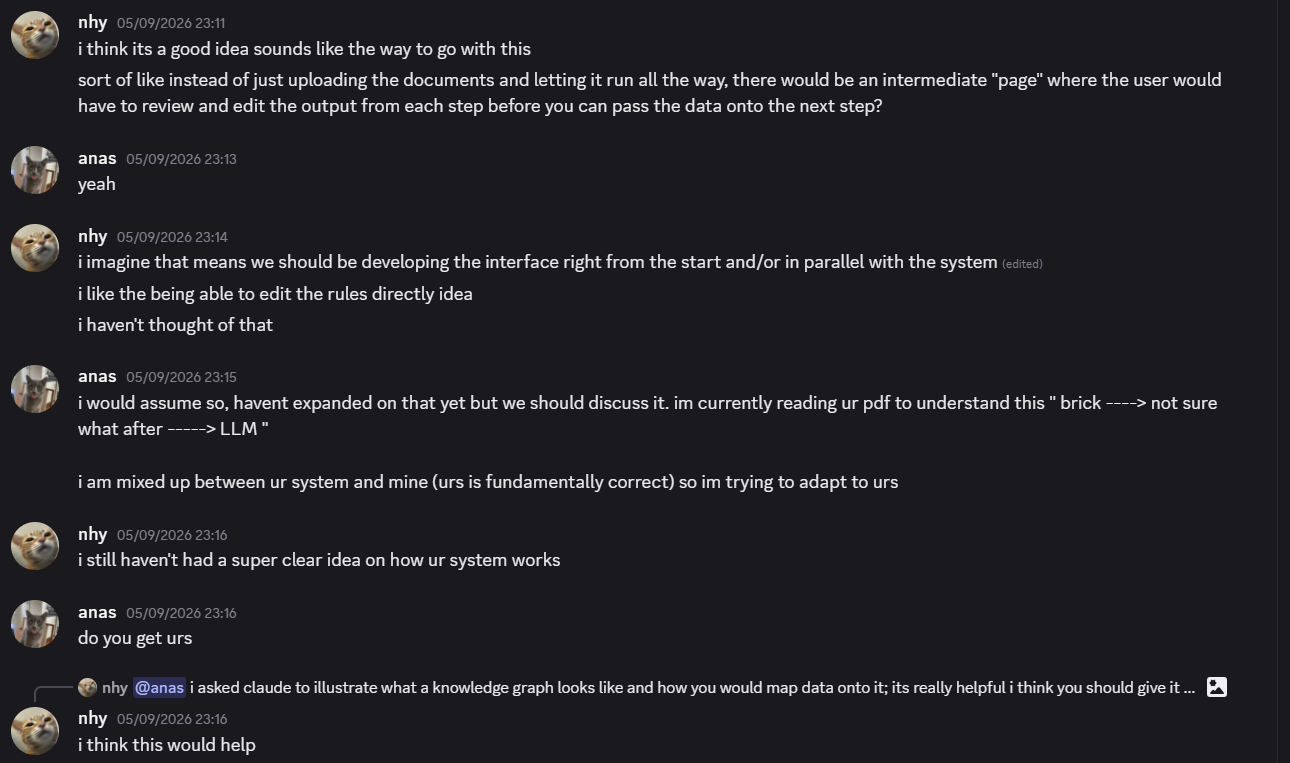
\includegraphics[scale=0.5]{images/8_discussion.jpg}
    \caption{One of the discussions I had with Anas about his model-agnostic design.}
    \end{figure}

\subsubsection*{Contribution 9 - Team and Project Plan Development and Submission}

    \begin{xltabular}{\textwidth}{p{2cm} X}
    \caption{Contribution 9 Details} \\
    \hline
    \textbf{STAR} & \textbf{Description} \\
    \hline
    \endfirsthead

    \hline
    \endlastfoot

    \textbf{Situation} & Our first group submission was the Team and Project Plan, due at the end of Week 6. This required us to allocate tasks between team members, set deadlines, and decide who would handle formatting, proofreading, and submission. \\

    \textbf{Task} & Allocate tasks to each member, establish deadlines, monitor progress throughout the week, and manage submission. \\

    \textbf{Action} & As team leader, I allocated tasks during one of our meetings by reviewing the rubric and the template, then asked members to volunteer for sections, with suggestions based on each person's strengths. Also as the main solution architect, I took on the Solution Approach and Research sections, which were shared with Anas. Since I thought Anas's other sections were quite heavy, we agreed I'd complete the Research section myself and he could add onto it if it felt necessary. \par Throughout the week, I checked in on team members' progress to make sure no one was falling behind, proofread and gave feedback on others' work, edited sections to improve overall quality, and helped with formatting the final submission. Krish was originally assigned to submit the plan, but couldn't due to work commitments, so I took on this task instead. \\

    \textbf{Result} & The team completed and submitted the plan well ahead of the deadline, with no last-minute issues or changes required, and the overall quality of the submission was strong. \\

    \end{xltabular}

    \begin{figure}[H]
    \centering
    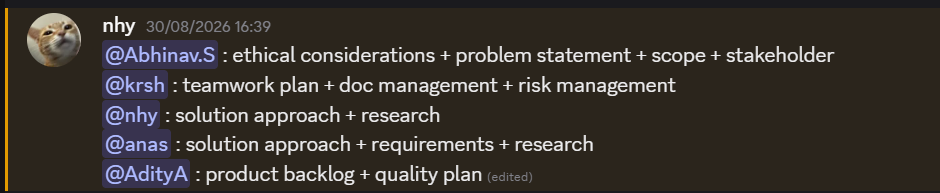
\includegraphics[scale=0.7]{images/9_tasks.jpg}
    \caption{Sections to complete by each member for the Team and Project Plan. This was also posted on Trello.}
    \end{figure}

    \begin{figure}[H]
    \centering
    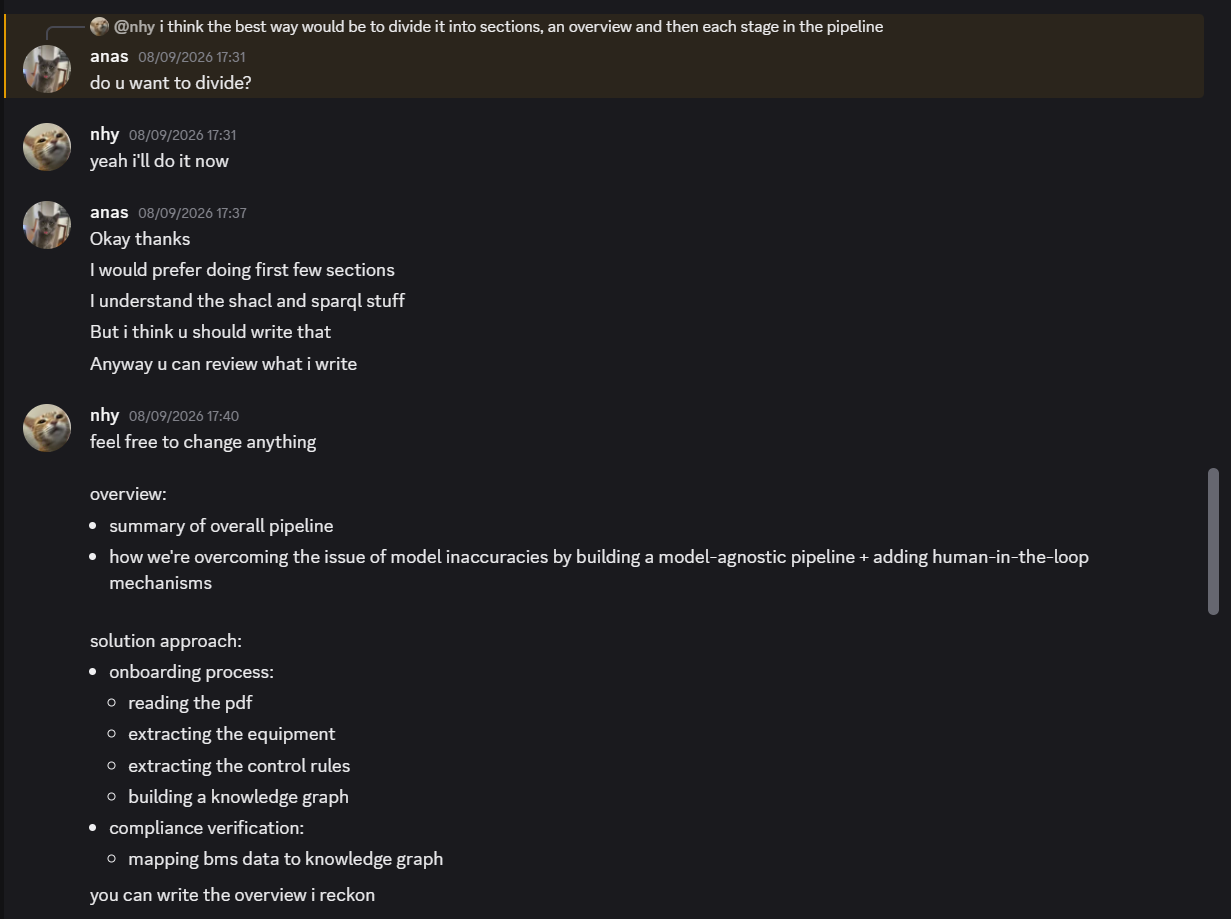
\includegraphics[scale=0.5]{images/9_divide_1.jpg}
    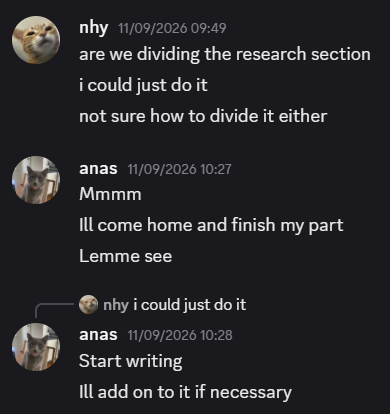
\includegraphics[scale=0.5]{images/9_divide_2.jpg}
    \caption{How Anas and I divided the sections shared between the two of us.}
    \end{figure}

    \begin{figure}[H]
    \centering
    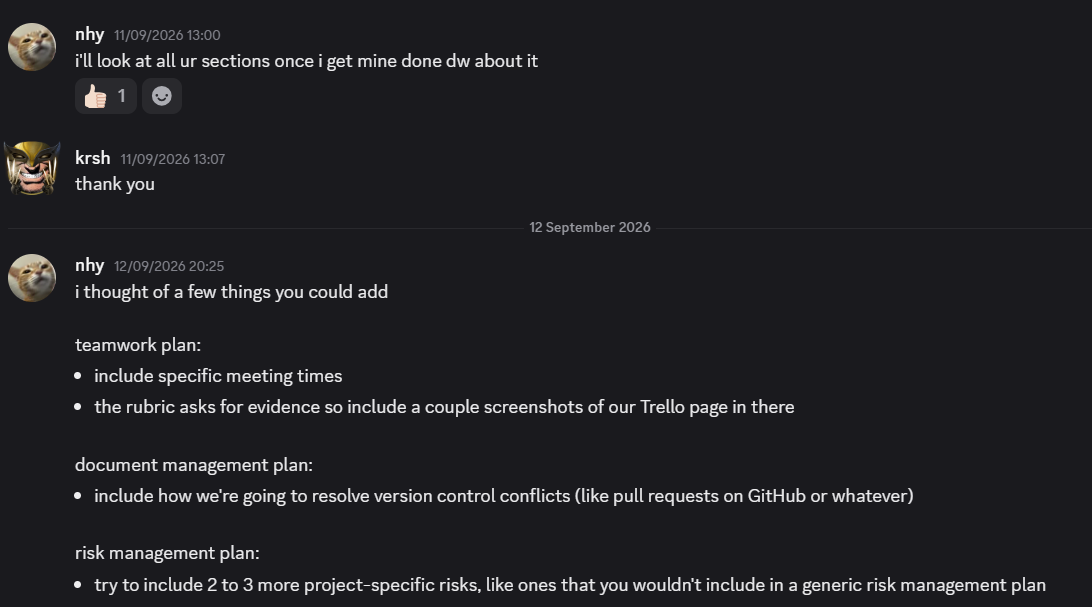
\includegraphics[scale=0.5]{images/9_feedback_1.jpg}
    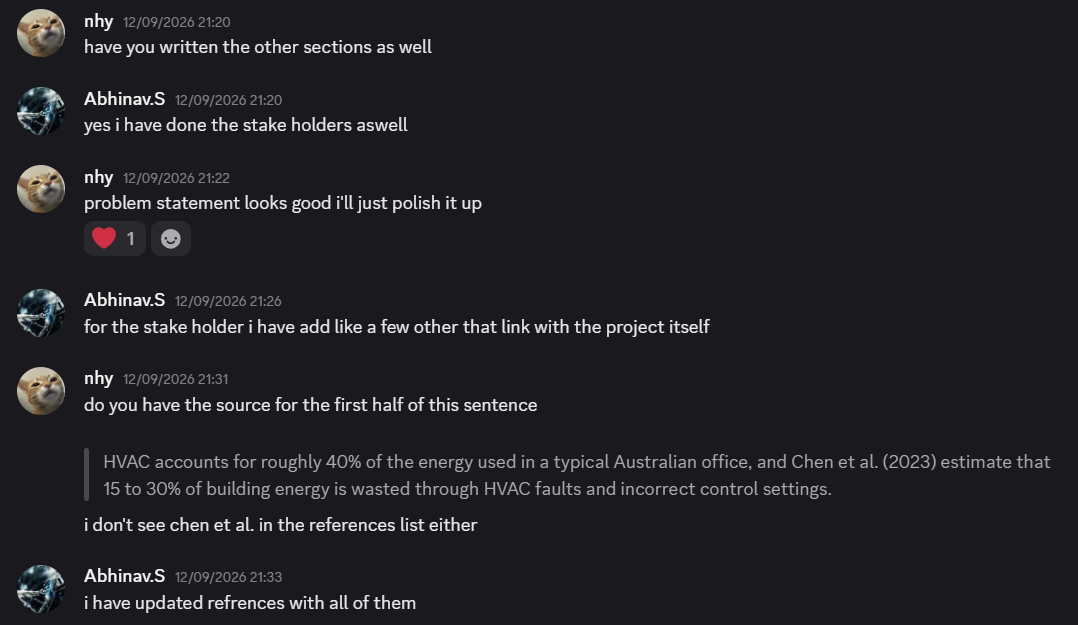
\includegraphics[scale=0.5]{images/9_feedback_2.jpg}
    \caption{I gave my feedback on my teammates' work when requested to.}
    \end{figure}

    \begin{figure}[H]
    \centering
    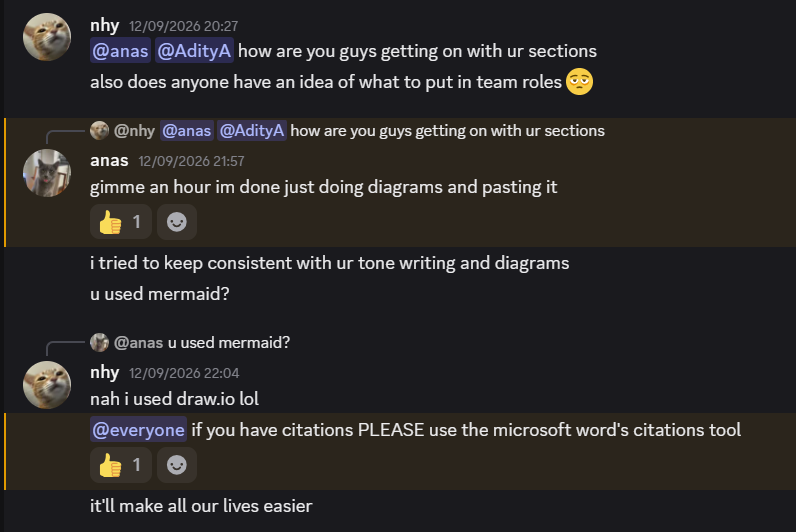
\includegraphics[scale=0.7]{images/9_checkin.jpg}
    \caption{Checking in on the team's progress.}
    \end{figure}

    \begin{figure}[H]
    \centering
    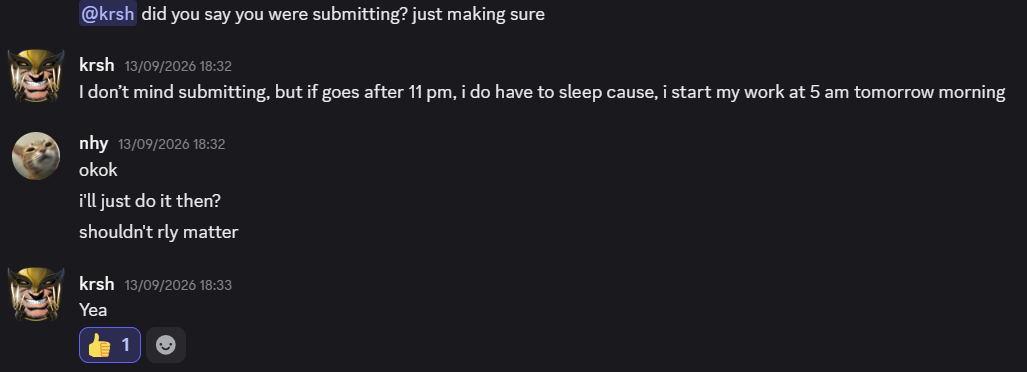
\includegraphics[scale=0.7]{images/9_submit.jpg}
    \caption{I offered to submit when Krish couldn't due to work obligations.}
    \end{figure}

\section{Teamwork, Communication, and Professional Practice}

\subsection{Engagement with Team Members}

Throughout this planning process, I stayed highly engaged with my team members. I often took the initiative to get the team started on tasks, organise team meetings, and coordinate responsibilities between team members. This can be seen throughout the screenshots of our Discord discussions and in our meeting notes. I believe that my level of involvement and proactiveness also contributed to me being elected as the team leader.

\begin{figure}[H]
\centering
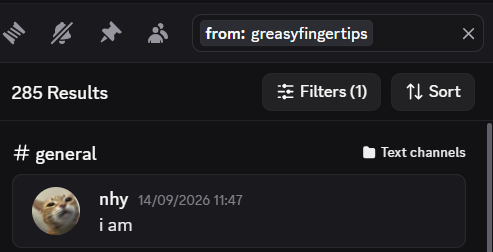
\includegraphics[scale=0.7]{images/messages.jpg}
\caption{I have sent 285 messages in the Discord chat since the start of our project, which proves that I have been engaging in our team discussions.}
\end{figure}

I participated in all team meetings except for one post-client-meeting debrief in Week 2, which I was unable to attend due to work commitments. I always stayed casual and friendly when communicating with the team, while still staying appropriate and professional when needed. I generally responded to other team members within a few hours or, at most, within the same day. I was also very involved in tasks which required collaboration with other members, especially towards the final few weeks of the planning process. When working with others, I made sure to gather everybody's opinions on matters before moving forward with decisions and provided constructive feedback when necessary. This is reflected in Contribution 9.

In retrospect, I think I could have been more direct and proactive during the first few weeks of meetings and discussions. Before we had an official team leader, I sometimes hesitated to take the lead, host meetings, or assign responsibilities. Looking back, I could have taken this initiative even before being officially designated the team leader. This would have given the team clearer direction right from the start and may have helped us progress more quickly.

\subsection{Engagement with the Supervisor and the Client}

I was also proactive when communicating with the other project stakeholders, including our supervisor and the project client. I contacted both stakeholders via email on behalf of the team in the first week of the project (Contribution 1). Throughout the planning phase, I participated in all supervisor and client meetings and regularly represented the team to discuss the progress we had made during the week. During these meetings, I also made an effort to stay professional by keeping my camera on and attending from an appropriate setting.

Table~\ref{tab:quick-links} provides hyperlinks to our meeting notes and client meeting recordings as evidence for my participation and engagement.

\begin{xltabular}{8cm}{p{4cm} X}
    \caption{Links to Meeting Notes and Recordings}
    \label{tab:quick-links} \\
    \hline
    \textbf{Type} & \textbf{Hyperlinks} \\
    \hline
    \endfirsthead

    \hline
    \endlastfoot

    \textbf{Notes} & \href{https://docs.google.com/document/d/1xmWgrOT3ej_nIsrpDg2PSpWdRceK8fwI6DNl7It1qHE/edit?usp=sharing}{Week 2} \par \href{https://docs.google.com/document/d/1WdaFi9pqphsC86g0fr1Vazsp2pVx1C348ypmlM1nFhQ/edit?usp=sharing}{Week 3} \par \href{https://docs.google.com/document/d/1KpA3DNGGgSsxD16WQFf-JHx9Obc0zjWh5djjO1siQ70/edit?usp=sharing}{Week 4} \par \href{https://docs.google.com/document/d/1cOQNOdxrQEmlKtBGA0fAi28BBBrSdBdxoyCWRU_OD2s/edit?usp=sharing}{Week 5} \par \href{https://docs.google.com/document/d/15exNUMa88fH8xraCrFS4MbCKsYV2SY9AaO6yHp1tKsk/edit?usp=sharing}{Week 6} \\

    \hline

    \textbf{Recordings} & \href{https://liveswinburneeduau-my.sharepoint.com/:v:/g/personal/mmalam_swin_edu_au/IQA-vwAUCcfORKNHUEILTop7AYi5FJB4q9DqV2oNC07e3mc}{Week 2} \par \href{https://liveswinburneeduau-my.sharepoint.com/:v:/g/personal/mmalam_swin_edu_au/IQAQdV7vCtFsRZlFDRKLair5AQq96RTto9ptNtQ1EkszQQQ}{Week 3} \par \href{https://liveswinburneeduau-my.sharepoint.com/:v:/g/personal/mmalam_swin_edu_au/IQCjHg1VxAKjQaX10gQMdS9mAZ9juOZA04vp-M-fZ73Fgbc}{Week 4} \par \href{https://liveswinburneeduau-my.sharepoint.com/:v:/g/personal/mmalam_swin_edu_au/IQDj6eS1vwvfRaAoC6pNkwIJAXDrSPCZBAvRowFNn4i_6m0}{Week 5} \par \href{https://liveswinburneeduau-my.sharepoint.com/:v:/g/personal/mmalam_swin_edu_au/IQBJRG8SwuqaQLh0AmcRBmMoAXVvGyhvHIAniya6kSLihTo}{Week 6} \\
\end{xltabular}

\section{Reflection, Learning, and Continuous Improvement}

\subsection*{What went well}

I am proud of the contribution I have made towards this project so far. I contributed significantly to the logistical organisation and coordination of the team, worked towards the final solution design, particularly through my collaboration with Anas, and ensured that our outcomes were delivered on time and to a good standard. I was also able to take on the role of team lead during this phase and help guide the team's direction. I believe this had a positive effect on keeping the team aligned and making sure we continued progressing towards our goals. 

\begin{figure}[H]
\centering
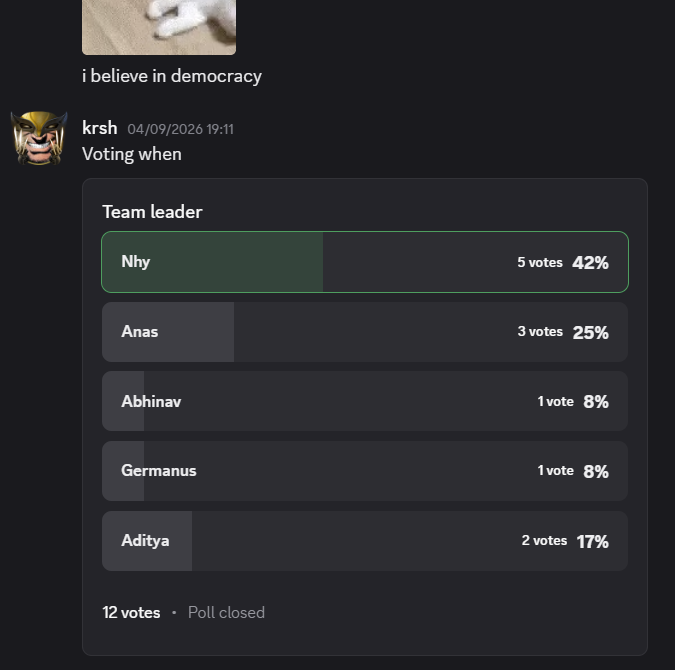
\includegraphics[scale=0.6]{images/team_lead.jpg}
\caption{I was voted to be the team lead by the other team members.}
\end{figure}

\subsection*{Challenges faced}

One of the main challenges I faced was keeping the team on the same page. This phase of the project was very research-heavy and required each team member to spend a significant amount of time learning and studying independently. As a result, it was difficult to ensure that everyone had the same understanding of the project and its requirements. This contributed to the team remaining undecided on parts of the project until the final stretch before the demonstration. I also felt that some of my research efforts were not fully understood by the other team members, which made it more difficult to use that research towards a shared understanding.

Another challenge was the level of initiation and input from other team members, particularly when developing the final architecture of the project. Since many aspects of the project were also new to me, I found it difficult to develop the architecture without having other ideas or proposals to compare against. This made me less confident in determining whether my own proposal was the most appropriate approach.

I also had a lot of difficulty balancing my project responsibilities with other commitments. At times, I had ideas or tasks that I wasn't able to fully realise because I had to prioritise other responsibilities. This meant that I had to focus on completing the most important components of a task rather than developing an idea as thoroughly as I would have liked to.

\subsection*{What I learned}

I learned that taking initiative early can give a team clearer direction, as I found that being more proactive with organisation and direction helped the team progress better once I became the team lead. This showed me that I do not necessarily need to wait for someone to formally assign me a leadership responsibility before taking initiative.

\subsection*{How I would apply this in the future}

In future projects, I would take a more direct and proactive approach right from the beginning. This means establishing clearer responsibilities, organising discussions, and helping the team agree on a direction earlier. This would reduce the uncertainty we experienced towards the end of this phase.

I would also make a greater effort to ensure that the team has reached a shared understanding. Since much of the research was new to all of us, having more in-depth technical discussions would allow team members to help each other progress in their research and keep everybody informed about the final decisions.

% References
% \printbibliography
\end{document}